\documentclass[a4paper]{article}
\usepackage{tikz}
\usetikzlibrary{petri,arrows}
\usepackage{amstext}

\begin{document}


%% TikZ style options %%
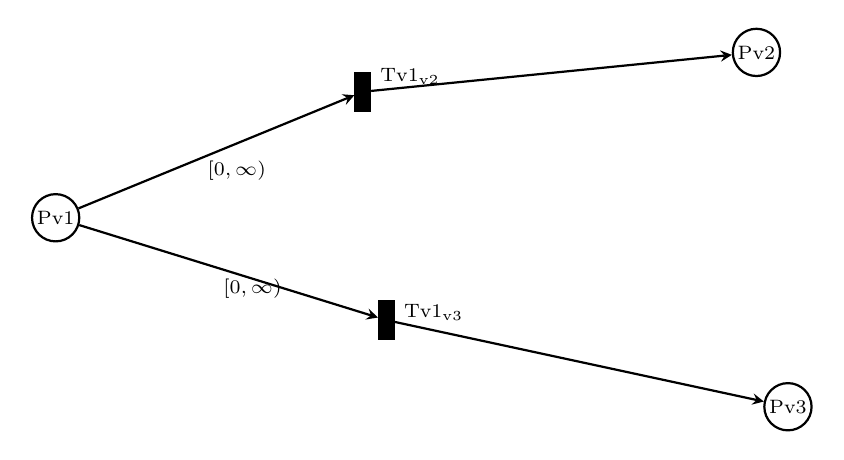
\begin{tikzpicture}[font=\scriptsize, xscale=1, yscale=1]
%% the figure can be scaled by changing xscale and yscale
%% positions of place/transition labels that are currently fixed to label=135 degrees
%% can be adjusted so that they do not cover arcs
%% similarly the curving of arcs can be done by adjusting bend left/right=XX
%% labels may be slightly skewed compared to the tapaal drawing due to rounding.
%% This can be adjusted by tuning the coordinates of the label
\tikzstyle{arc}=[->,>=stealth,thick]
\tikzstyle{transportArc}=[->,>=diamond,thick]
\tikzstyle{inhibArc}=[->,>=o,thick]
\tikzstyle{every place}=[minimum size=6mm,thick]
\tikzstyle{every transition} = [fill=black,minimum width=2mm,minimum height=5mm]
\tikzstyle{every token}=[fill=white,text=black]
\tikzstyle{sharedplace}=[place,minimum size=7.5mm,dashed,thin]
\tikzstyle{sharedtransition}=[transition, fill opacity=0, minimum width=3.5mm, minimum height=6.5mm,dashed]
\tikzstyle{urgenttransition}=[place,fill=white,minimum size=2.0mm,thin]\tikzstyle{uncontrollabletransition}=[transition,fill=white,draw=black,very thick]
%% TikZ-figure elements %%
\node[place] at (1.8,-4.7) (Pv1) {};
%% label for place Pv1
\draw (1.8,-4.7) node[align=left] {$\mathrm{Pv1}$};
\node[place] at (10.7,-2.6) (Pv2) {};
%% label for place Pv2
\draw (10.7,-2.6) node[align=left] {$\mathrm{Pv2}$};
\node[place] at (11.1,-7.1) (Pv3) {};
%% label for place Pv3
\draw (11.1,-7.1) node[align=left] {$\mathrm{Pv3}$};
\node[transition] at (5.7,-3.1) (Tv1_v2) {};
%% label for transition Tv1_v2
\draw (6.3,-2.9) node  {$\mathrm{Tv1_{v2}}$};
\node[transition] at (6.0,-6.0) (Tv1_v3) {};
%% label for transition Tv1_v3
\draw (6.6,-5.9) node  {$\mathrm{Tv1_{v3}}$};
\draw[arc] (Pv1) to[bend right=0] (Tv1_v2) {};
%% Label for arc between Pv1 and Tv1_v2
\draw (4.1,-4.1) node {$\mathrm{[0,\infty)}$};
\draw[arc] (Tv1_v2) to[bend right=0] (Pv2) {};
\draw[arc] (Pv1) to[bend right=0] (Tv1_v3) {};
%% Label for arc between Pv1 and Tv1_v3
\draw (4.3,-5.6) node {$\mathrm{[0,\infty)}$};
\draw[arc] (Tv1_v3) to[bend right=0] (Pv3) {};
\end{tikzpicture}
\end{document}
